\section{Architekturkonzept}
\label{sec:architekturkonzept}
    Das Framework stellt die Kern-Funktionalität zur Steuerung von implementierten Regeln und Prozessen innerhalb eines 
    Gebäudes, bspw. eines Büroraumes, dar. Mit dem Architekturkonzept wird der grundlegende Aufbau, sowie die Funktionalität des Frameworks erläutert. 
    Potentielle Erweiterungen und Adaptionen werden im Ausblick (\ref{chap:ausblick}) aufgegriffen.
    \\ 
    \linebreak
    Das System soll in drei Schichten aufgeteilt werden. Die oberste Schicht stell die Kommunikationsschicht dar, die mittlere Ebene 
    handelt um die Logik- und Prozessschicht und der unterste Block repräsentiert die Persistenzschicht. Im Rahmen der Arbeit wird 
    die dritte Schicht nicht weiter konkretisiert, da diese zu aktuellem Zeitpunkt keinen Nutzen generiert, bzw. für keine weitere Verarbeitung 
    genutzt wird. Die Ausprägung der Schicht ist dennoch ohne weiteres möglich und wird auch grob skizziert. Der Abbildung 
    (\ref{fig:schichtenarchitektur}) ist die Aufteilung der Schichtenarchitektur zu entnehmen. In der Darstellung unterscheidet sich die 
    Persistenzschicht von den anderen, um erkenntlich zu machen, dass diese in aktuellem Konzept lediglich eine Nebenrolle spielt. 
    Durch die Darstellung in übergreifender Form wird deutlich, das bereits auf dieser Ebene die Trennung der Zuständigkeiten, engl. 
    \textit{seperation of concerns}, greift. Durch die gezielte Abstraktion von Komponenten und Informationen kann die Komplexität 
    eines Systems gesteuert werden. Die Kommunikationsschicht ermöglicht die Anbindung von verschiedensten Kommunikationsprotokollen, die 
    dadurch schnell adaptiert werden können. Im Rahmen des Konzeptes wird ausschließlich Gebrauch des \acs{MQTT}-Protokolls gemacht. 
    Die Logikschicht nimmt alle eingehenden Events, die jeweils eine Zustandsänderung erzwingen, der Kommunikationsschicht entgegen 
    und durchläuft den Prozess des Frameworks, um auf die Zustandsänderung die passende Regel auszuführen. Die 
    Persistenzschicht ist für die Speicherung erzeugter Daten zuständig, bspw. wenn eine Transaktionshistorie von Zustandsänderungen 
    persistiert werden soll. Ebenso können Informationen gespeichert werden, die anderweitig zur Verfügung stünden.  
    \begin{figure}[hbt!]
        \centering
        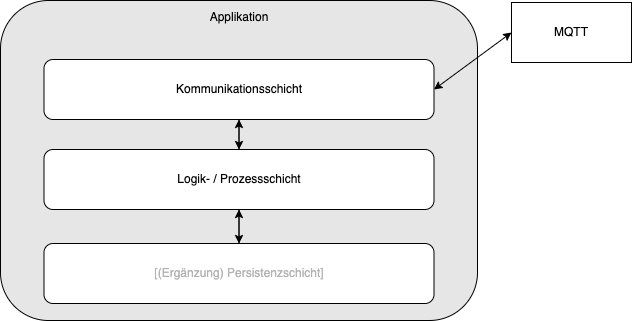
\includegraphics[width=14cm,height=10cm,keepaspectratio]{images/Schichtenarchitektur.png}
        \caption{Schichtenarchitektur}
        \label{fig:schichtenarchitektur}
    \end{figure}
    \\
    %\pagebreak
    Für die Konzeption von wartbarer und erweiterbarer Software, wird von den \textit{SOLID}-Prinzipien, sowie von nützlichen 
    und für das Framework verwendbaren Programmiermustern Gebrauch gemacht. Diese werden an geeigneter Stelle und auf den Nutzen bezogen erläutert.
    \\
    \linebreak
    Das \textit{SOLID} wurde von Robert C. Martin\footnote{Software Engineer, Lehrer und Autor Robert C. Martin. \url{https://en.wikipedia.org/wiki/Robert_C._Martin} Besucht am 10.07.2022} 
    geprägt und soll zum Design guter objektorientierter Software beitragen. Dadurch soll 
    ein Softwaresystem einer höheren Wartbarkeit unterliegen. Es setzt sich aus fünf Prinzipien zusammen, die wie folgt definiert sind.
    \begin{itemize}
        \item S - Single-Responsibility-Prinzip: „Das Single-Responsibility-Prinzip (SRP; Eine-Verantwortlichkeit-Prinzip; ...) fordert, dass eine Klasse oder ein Modul einen und nur einen \textit{Grund zur Änderung} haben sollte.“ \cite{cleancode2009}
        \item O - Open-Closed-Prinzip: „Module sollten sowohl offen (für Erweiterungen) als auch verschlossen (für Modifikation) sein.“ \cite{ocpmeyer1988}
        \item L - Liskovsches Substitutionsprinzip: „... Sei q(x) eine beweisbare Eigenschaft von Objekten x des Typs T. Dann soll q(y) für Objektes des Typs S wahr sein, wobei S ein Untertyp von T ist.“ \cite{liskov2001behavioral} - Das (Ersetzungs-)Prinzip sagt somit aus, dass eine 
        Subklasse stets die Eigenschaften der Superklasse erfüllt und immer als Objekt der Superklasse anwendbar sein muss. Eine Subklasse darf dadurch erweitert werden, aber 
        keine grundlegende Änderung erfahren. 
        \item I - Interface-Segregation-Prinzip: „Clients sollen nicht dazu gezwungen werden, von Interfaces abzuhängen, die sie nicht verwenden.“ \cite{martin1996interface}
        \item D - Dependency-Inversion-Prinzip: „A. Module hoher Ebenen sollten nicht von Modulen niedriger Ebenen abhängen. Beide sollten von Abstraktionen abhängen. B. Abstraktionen sollten nicht von Details abhängen. Details sollten von Abstraktionen abhängen.“ \cite{martin2003agile}
    \end{itemize}
    Diese Prinzipien werden bei der Konzeption des Frameworks berücksichtigt. Da es sich bei diesem System nicht um eine klassische 
    Webanwendung handelt und keine direkte Kommunikation unter anderem über \acs{REST} \acs{API}s stattfindet, wird ein allgemeines 
    Programmiermuster, wie bspw. das \ac{MVC}\footnote{Architekturmuster für Webapplikationen. \url{https://de.wikipedia.org/wiki/Model_View_Controller} Besucht am 10.07.2022} 
    oder das \ac{MVVM}\footnote{Software-Architekturmuster. \url{https://en.wikipedia.org/wiki/Model–view–viewmodel} Besucht am 10.02.2022 }, nicht 
    in Betracht gezogen. Verwendet werden allgemeine Architekturmuster und -prinzipien, die dazu beitragen die Software wartbar 
    zu gestalten, die Komplexität einzelner Funktionen zu reduzieren und die Lesbarkeit und Überschaubarkeit zu erhöhen. 
    
    \subsection{Generische Programmierung} % Typisierung
        % Erledigt! -> WICHTIG!!!: Verwendung der Typisierung, um dem Anwender die Möglichkeit der offenen Gestaltung des Zustandobjektes zu gewährleisten.
        Eine entscheidende konzeptionelle Überlegung in Richtung des Zustandsraumes wird vorab erläutert, damit in 
        folgenden Darstellungen klar zwischen der Objektdarstellung und der eigentlichen Repräsentation des Zustandes 
        differenziert werden kann. 
        \\
        Mit dem Hintergrund, dass der Entwickler die volle Entscheidungsmacht über die Implementierung der 
        Regeln, des Zustandsraumes und den dafür notwendigen Bedingungen beibehält, ist die Überlegung  
        notwendig, wie mit einem Objekt gearbeitet werden kann, ohne dass es vorher bekannt ist. 
        \\
        \linebreak
        Hierfür wird auf das Konzept der generischen Programmierung, sog. \textit{Generics}, gesetzt. Ein Synonym 
        des Begriffs ist der parametrisierte Typ. Mit der Nutzung von Generics ist ein syntaktisches Mittel 
        gegeben, mit dem Klassen und Methoden mit Typen parametrisiert werden können. Diese Typ-Variablen sind zum 
        Zeitpunkt der Implementierung unbekannt und können beliebig definiert werden. Erst zur Laufzeit des Systems 
        wird die Typ-Variable durch einen oder ggf. auch mehrere Typen ersetzt. Somit ist zur Laufzeit das 
        Objekt, dessen Struktur, Methoden und Funktionen bekannt. Bei der Verwendung von generischen Typen gibt es 
        Varianzfälle, die unterschiedliche Auswirkungen aufzeigen. Der für das Konzept relevante Fall ist der des 
        einfachen Typ-Parameters. Weitere Varianzfälle werden in dieser Ausarbeitung nicht erläutert. 
        \\
        \linebreak
        Ein konkretes Anwendungsbeispiel, wie es 
        auch im Rahmen dieser Arbeit verwendet wird, sieht wie folgt aus:
        \\
        Das Framework arbeitet mit dem generischen Typ \textit{E}. Der Anwender soll nach der Implementierung der Klasse des Zustandsraumes das 
        jeweilige Objekt dem Framework übergeben. So ist zur Laufzeit das konkrete Objekt bekannt. Zur Veranschaulichung dient folgendes Code-Beispiel:
\begin{lstlisting}[language=Java, frame=lines, xleftmargin=\parindent, style=algoBericht, label={code:generics}, captionpos=b, caption={Zustandsobjekt als Typ-Variable}]
public class LogicHub<E> {
    private E state;
    ...
    public E getState() {
        return this.state();
    }
    ...
}

public class Application {
    private final LogicHub<InnovationLab> logicHub;

    public static void main(String[] args) {
        logicHub = LogicHub.getInstance();
        logicHub.getState(); // -> returns the InnovationLab object 
                             // and it's values.
        ...
    }
}
\end{lstlisting}
        Mit den Java Generics ist eine leistungsstarke Ergänzung der Java-Sprache gegeben, da es die Arbeit des Programmierers einfacher und 
        weniger Fehleranfällig macht. Zusätzlich wird durch die Generics die Typkorrektheit zur Kompilierzeit erzwungen und ermöglicht 
        die Implementierung generischer Algorithmen, ohne für Anwendungen einen zusätzlichen Overhead zu verursachen. 
        \\
        Mit der Option des generischen Typs kann das Framework universell definiert und der Zustandsraum vom Anwender individuell implementiert werden.
        \\
        \linebreak
        Die Darstellung des Zustandsobjektes wird als bereits bestehendes vorausgesetzt, um die folgenden Diagramme vollständig und sinngemäß wiederzugeben. 
        Diese beschreiben jedoch zu keinem Zeitpunkt eine konkrete Struktur. 
        \\
        \linebreak
        Im weiteren Verlauf wird der Aufbau der Komponenten erläutert, sowie die einzelnen Schichten und deren Funktionalitäten näher beschrieben.

    \subsection{Aufbau der Komponenten}

    

    % ALLGEMEIN MIT PATTERNS BESCHREIBEN (KERN-KOMPONENTEN UND DARAUF ANGEWENDETE PATTERN)
    \subsection{Kommunikationsschicht}

    % NOCHMALS DIE SCHICHTEN MIT:
    % KOMMUNIKATIONSSCHICHT UND AUFBAU -> \subsection{}?

    \subsection{Logik- und Prozessschicht}
    % LOGIKSCHICHT UND AUFBAU -> \subsection{}?

    \subsection*{Persistenzschicht}
    % EVTL.: PERSISTENZSCHICHT UND POTENTIELLER AUFBAU -> \subsection{}?

    % Es wird alles abgebildet über einen Zustandsraum, der sich aus den Dingen (Gegenständen) und Zuständen der Anwendung ergibt.
    % Der Zustandsraum wird verändert, wenn eine Aktion durchgeführt wird, bzw. durch eine Trigger angestoßen. 
    % Bzw. speichert den aktuellen Zustand des Gegenstandes 
    % (lightBulb = true/false, personOnDoor = null/Mikka, booking = stringBooking, temiAktive = true/false, 
    % temiPosition = stringKoordinates)
    % Zustandsraum muss von dem Entwickler definiert werden. 
    % MQTT Broker über Home Assistant, bzw. losgelöster Broker
    % Anbindung von APIs auch Entwickler-Sache. Kann ich das vereinfachen, sodass die Integration einfacher wird?

    \subsection{Überlegungen, Anstöße und Herausforderungen}
    % Regeln über Thread abbilden? Ja, Nein? - Nein, wieso? Da Durch die MQTT Message mehrere Regeln ausgeführt 
    %werden können. -> Lediglich den Zustand der Komponenten locken.
    % KEIN THREAD (wird schon abgebildet durch die Services und die Auslöser durch MQTT), Falls eine Komponente 
    %  doppelt beansprucht wird, ist der Zustand der Komponenten zu locken und ein 
    % Thread.sleep einzurichten. Abfrage, ob der Wert, bzw. die Komponente wieder freigegeben wurde. 

    % Zustandsraum -> Abbildung aller notwendigen Komponenten 
    % Bei Bearbeitung einer Regeln die Komponenten Locken, sodass nur die einzelne Komponenten (deren Zustand) gelockt ist 
    % und nicht der ganze Zustandsraum, somit können mehrere Komponenten und Aktionen ausführen zu können. 

    %Was brauche ich für Funktionen und Werte in einer Regel?

    % Ein Zustandsraum (Objekt) für alles oder ein Globales, welches die die Komponenten enthält? - Begründung für die Auswahl.
    
    %\subsection{Schnittstellen}
        % Kommunikation mit API's je nach Use Case und Gebrauch zur Datenabfrage
    
    %\subsection*{Datenbanken}
    %   Anbindungen an Datenbanken sind je nach hinzukommendem Anwendungsfall ohne weiteres möglich. Dies ist eine Konzeptvertiefung, die 
    %    im Rahmen dieser Arbeit nicht konkretisiert wird, da der Fokus auf der Kernfunktionalität, sowie auf dem 
        % Datenbanken je nach Use Case und Gebrauch zur Datenabfrage

    \subsection{Parallelität}


    %HERAUSFORDERUNG MIT DEM QUEUEING ANTEASERN.

\subsection{Softwarekonzept}
\label{subsec:softwarekonzept}



